\section{\textbf{Our Approach}}\label{sec:main}
\subsection{ Proposed Solution}

This project was developed in Javascript programming language to be able to use hls-parse js library features, with Node JS and npm as deployment and distribution tools. 

We parsed the HLS manifests from the multiple input video streams using the hls-parse JS library. Having the respective object representations for further manipulation and handling, we implemented two algorithms that identify the matching representations based on resolution, shown in Figure \ref{fig:strategies}.

 \begin{itemize}

     \item Strategy 1: The first strategy consists of identifying which video streams have matching representations against the first element of the input array. One video stream might have more resolutions than the first input so those would be left out. As can be seen in Figure \ref{fig:strategies}, video stream B does not have the green resolution, that is present in A, so this stream is not present in the final output.

     \item  Strategy 2: The second strategy consists of finding an intersection between the variant playlists in regards to their resolution. In Figure \ref{fig:strategies} we can see that only two resolutions are common between all the input streams so an intersection has been found. Two variant playlists should be in the output manifest. Each one will include all concatenated segments from all inputs matching the respective representation.


 \end{itemize}
 
 For both strategies, the final output should be the master HLS manifest of a playlist that includes the concatenated segments from all inputs matching the respective representation. Using the hls-parser library we will create and manipulate this final HLS master manifest.

 
\begin{figure}[!ht]

\centering
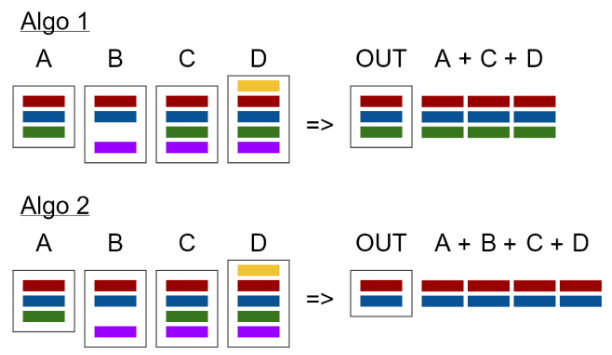
\includegraphics[scale=0.70]{figures/strategies.png}
\caption{Strategies}
\label{fig:strategies}
\end{figure}

In figure \ref{fig:proposal} we can see the diagram flow that shows how the multiple video streams manifest as input are going to be parsed through the hls-parse library to obtain each object representation, so we can handle and manipulate its data. Then, the two strategies will be applied to this set of objects to find the matching and compatible representations to output a final master playlist using, again, the hls-parse library to create/write the master manifest.

\begin{figure}[!ht]

\centering
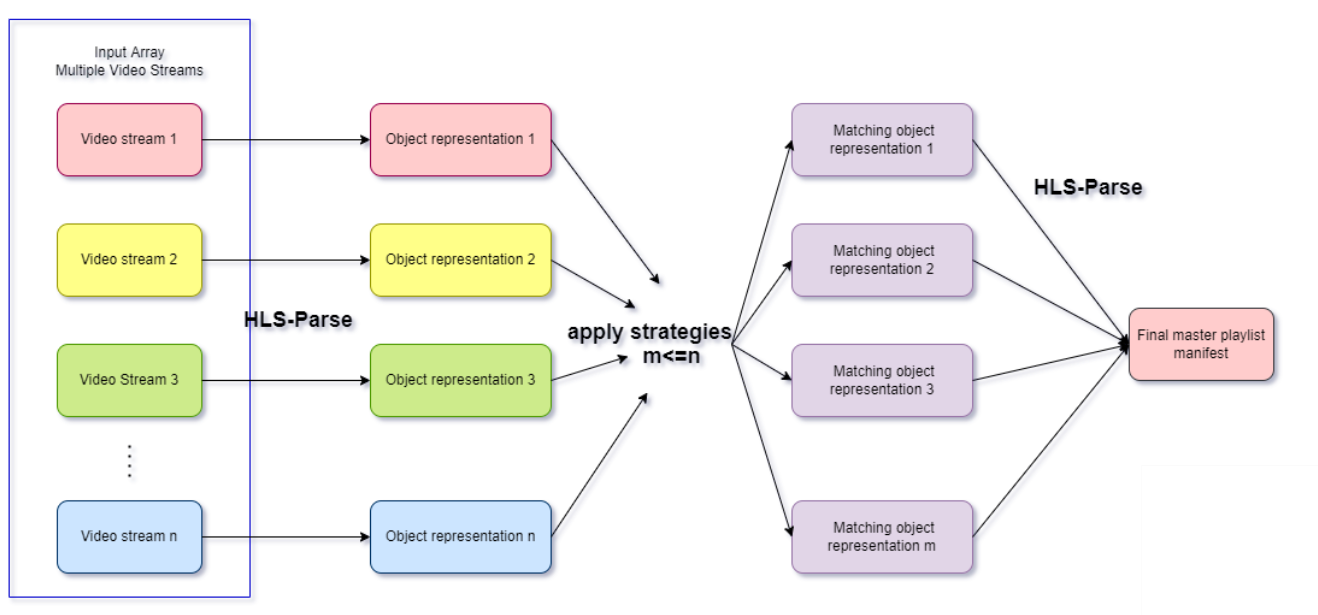
\includegraphics[scale=0.31]{figures/proposal.png}
\caption{Proposed Solution}
\label{fig:proposal}
\end{figure}

\subsection{HLS Manifest Parsing}

Each strategy receives as a parameter an array made of Strings consisting of different video stream URLs that are already .m3u8 files. To obtain the manifest text from the URLs, we fetched the data using the \Verb|fetch()| JavaScript function, which makes a GET request to the URL to obtain the text data returned. Then, we parsed the text into object representation using the hls-parser library to access the playlist as a JS object.

Hls-parser provides synchronous functions to read/write HLS playlists \cite{hlsparser}. With the method \Verb|HLS.parse(string)|, we obtained the Master playlist manifest from each URL. The object representation of a Master Playlist, its Variants, and audio tracks, look like this (simplified):

\begin{lstlisting}

MasterPlaylist {
  type: 'playlist',
  isMasterPlaylist: true,
  uri: 'https://playertest.longtailvideo.com/adaptive/elephants_dream_v4/redundant.m3u8',
  version: 3,
  source: '#EXTM3U\n' +
    '#EXT-X-MEDIA:TYPE=AUDIO,GROUP-ID="aac",LANGUAGE="en",NAME="English",DEFAULT=YES,URI="media/b160000-english.m3u8"\n' +
    '#EXT-X-STREAM-INF:BANDWIDTH=2962000,RESOLUTION=1280x720,AUDIO="aac"\n' +
    'media/b2962000-video.m3u8\n' +
    '#EXT-X-STREAM-INF:BANDWIDTH=1427000,RESOLUTION=768x432,AUDIO="aac"\n' +
    'media/b1427000-video.m3u8\n',
  variants: [
    Variant {
    uri: 'media_b/b2962000-video.m3u8',
    bandwidth: 2962000,
    resolution: { width: 1280, height: 720 },
    audio: [ 
    Rendition {
      type: 'AUDIO',
      uri: 'media/b160000-english.m3u8',
      groupId: 'aac',
      language: 'en',
      assocLanguage: undefined,
      name: 'English',
      isDefault: true,
      }
    ]
  },
    Variant {
    uri: 'media_b/b1427000-video.m3u8',
    bandwidth: 1427000,
    resolution: { width: 768, height: 432 },
    audio: [ 
    Rendition {
      type: 'AUDIO',
      uri: 'media/b160000-english.m3u8',
      groupId: 'aac',
      language: 'en',
      assocLanguage: undefined,
      name: 'English',
      isDefault: true,
      }
    ]
  }
  ],
}

\end{lstlisting}

The resolution attribute from the Variant object will be useful in finding the matching representations for each strategy. The bandwidth attribute helped us choose which representation to include when two shared the same resolution but with different bandwidths, taking the highest one. The different Uri attributes are concatenated at the end of the original address of the master playlist to later fetch the text data inside those .m3u8 files for Variant and Audio playlists.

Having the complete object representation, we saved the different Variants from each URL into a Dictionary, where the key is the index of the URL in the input URLs array and has as value an array made of the variants objects from that stream. We also saved the object representation from all the playlists in another array for later use.

\subsection{Strategy 1}

We need as a final output a master playlist that contains the same representations available from the first video stream of the input array. So, if we have as input array [urlA, urlB, urlC], where stream A has 360p  and 720p resolutions, stream B has 360p, 480p and 720p, and stream C has only 360p. The only stream that matched Stream A's representations was Stream B, so the final output will have Streams A and B content with 360p and 720 representations. 

We extracted the resolutions of the first element of the array from the variants dictionary mentioned before. These are our needed resolutions, then we will iterate over the other streams and for each, we will obtain its variants. We will find the needed resolution in all the representations available for every other stream. We will save the object representation of the matching streams into an array for later use.

\subsection{Strategy 2}

For strategy 2 we have as output a master playlist that contains the representations resulting from the intersection, if one exists, of all the streams variants. From the variants dictionary, we get the representations for each stream, making an array of arrays. Then, for every stream representation, we check if it exists in every other stream variant. The number of times a representation appears in the other streams to be in the intersection should equal the number of video streams minus one. If no representation is present in every stream, the intersection is empty.

So, if we have as input array [urlA, urlB, urlC], where stream A has 720p and 360p resolutions, stream B has 480p and 360p and stream C has only 360p, an intersection exists and the Master Playlist will consist of only the 360p representation of Stream A, B and C contents.

\subsection{Output final master manifest}

After implementing both strategies, we have as a result an array with the compatible streams and an array with the resolutions that matched.
Having the streams resulting from the filtering of the strategies, we have to obtain the variants for each matching resolution.

With the help of a dictionary with key the resolution as string representation in 00x00 format, we gather all the variants that matched it according to the strategy. A stream can have multiple variants with the same resolution but with different bandwidths. To remove these duplicates, we chose the variant with the maximum bandwidth value.

For each matching resolution, we fetch the media playlist of all the variants to obtain their segments which will be joined in an array to create a new Media Playlist object that will represent the correspondent Variant representation in the final master manifest. We convert this new Media Playlist object into string representation in a .m3u8 file identified with the corresponding resolution using \Verb|HLS.stringify()| method.

\begin{lstlisting}
let newPlaylist = new MediaPlaylist({
    segments: segments,
    endlist: true,
    targetDuration: maxDuration,
    version: maxVersion
})
const content = HLS.stringify(newPlaylist)
fs.writeFile(resolution + '.m3u8', content)
\end{lstlisting}

Then, we create a new Variant object that has as Uri attribute the filename of the media playlist m3u8 file mentioned before, its resolution, and bandwidth attributes, which is the maximum of all the variants joined. This new Variant object will be saved in the variants dictionary mentioned before in the corresponding resolution key as 00x00 format.

\begin{lstlisting}
let newVariant = new Variant({
    uri: resolution + '.m3u8',
    resolution: res,
    bandwidth: maxBand
})
repDict[resolution] = newVariant
\end{lstlisting}

If the matching streams have audio tracks, these will also be fetched from the correspondent .m3u8 files of the audio media playlist. Each audio segment will be saved in an array, accumulating audio from all the streams belonging to a Variant. The attribute audio for the new Variant object will have as value this audio segments array. At the same time, a new audio.m3u8 file is written which will include the audio for the final resulting stream. 
\begin{lstlisting}
let newAudioPlaylist = new MediaPlaylist({
    segments: audioSegments,
    endlist: true,
    targetDuration: maxAudioDuration,
    version: maxAudioVersion
})
const content = HLS.stringify(newAudioPlaylist)
fs.writeFile('audio.m3u8', content)
let audio = new Rendition({
    type: 'AUDIO',
    uri: 'audio.m3u8',
    groupId: 'audio',
    name: 'audio'
})
newVariant.audio = [audio]
\end{lstlisting}
Finally, we create a new MasterPlaylist object joining all the variants in the dictionary in an array to assign the variants attribute to the master playlist. We convert this playlist into string representation too and write it on a master.m3u8 file.

\begin{lstlisting}
let masterPlaylist = new MasterPlaylist({
    variants: variants
})
HLS.stringify(masterPlaylist)
fs.writeFile('master.m3u8', content)
\end{lstlisting}

\subsection{Dependency Library}

The final requirement for this project was to deploy it as a dependency for other Node JS applications to use.

We created a npm package \cite{npm}, which has in the file utils.js two methods: \Verb|algorithmA()| and \Verb|algorithmB()|, where both receive as parameters an array of string URLs, along with other utility functions like \Verb|joinSegments()|, \Verb|makeRepresentationsDict()|, \Verb|createMasterPlaylist()|. These two methods, \Verb|algorithmA()| and \Verb|algorithmB()|, are exported in the index.js of the package from which an external Node JS app can import them as a dependency.